\chapter{General Analysis and Design}
\label{chap:general_analysis}
Before implementing the system a good design must be chosen. The design should be based on thorough analysis and discussion of alternative solutions.

This chapter deals with the analysis and design of the system. First the context of the final system is stated. Then the requirements specification is broken down and an analysis mixed with a design discussion is given for each requirement.

The chapter concludes with a summary of the chosen design and an overview of its main components.

\section{Context}
To design the system it is crucial to know the context of it.

\textbf{The satellites Failsafe Mode (FS)} \\
The failsafe program on the satellite is basically a request-response loop. Requests and responses are simple binary formatted streams of data. The failsafe commands and their formats are listed in appendix B.

\textbf{Ground Station (GS)} \\
When orbiting earth, communication with the satellite goes through a radio. This radio is controlled by a computer called the Ground Station. GS runs a UNIX variant as operation system. To operate the failsafe mode communication must therefore go through the Ground Station computer.
There is a protocol layer for the datalink that must be used for communication with the radio.

\textbf{The staffs desktop computers} \\
The software must be operational from the staffs desktop computers.

\section{Analysis and design discussion}
In the follow each requirement is analysed. Challenges and possible solutions are discussed along the way.

The analysis is of an iterative nature. For each iteration the overall design will be enhanced to incorporate the requirement.

\subsection{Console program - FSClient}
We could solve this requirement with a console program named fsclient running on the Ground Station. Fsclient could take a satellite command and its arguments as parameters and send it via the radio interface of the Ground Station to the statellite. This is basically how fsclient for the DTUSat-1 works.

As fsclient would be installed on the Ground Station the staff members must use the physical computer or have access to it via SSH for instance.

\begin{figure}[h!] \centering
	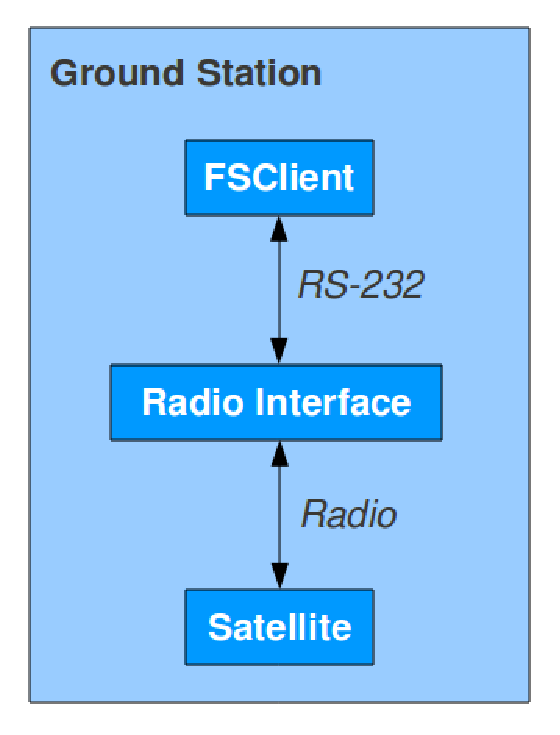
\includegraphics[scale=0.5]{img/interaction_via_console}
  \caption{FSClient on the Ground Station}
\end{figure}

\subsection{GUI}
There are many posibilities when it comes to implementing a GUI but regardless of the choice there must be communication with the satellite over the radio.

One way to solve this is to let the GUI connect to the Ground Station via SSH and use fsclient each time it must send a failsafe request.

A drawback to this solution is that not all GUI frameworks and operating systems have support for SSH out of the box.

\subsection{TCP Interface to the radio}
Alternatively there could be a TCP server on the Ground Station that listens for failsafe commands from connected TCP clients and have them forwarded to the radio. With this TCP server, called fsserver, we effectively have a TCP interface to the satellite and the advantage here is that all major GUI frameworks and all major operating systems have TCP support making this solution far more flexible than the SSH solution.

\begin{figure}[h!] \centering
	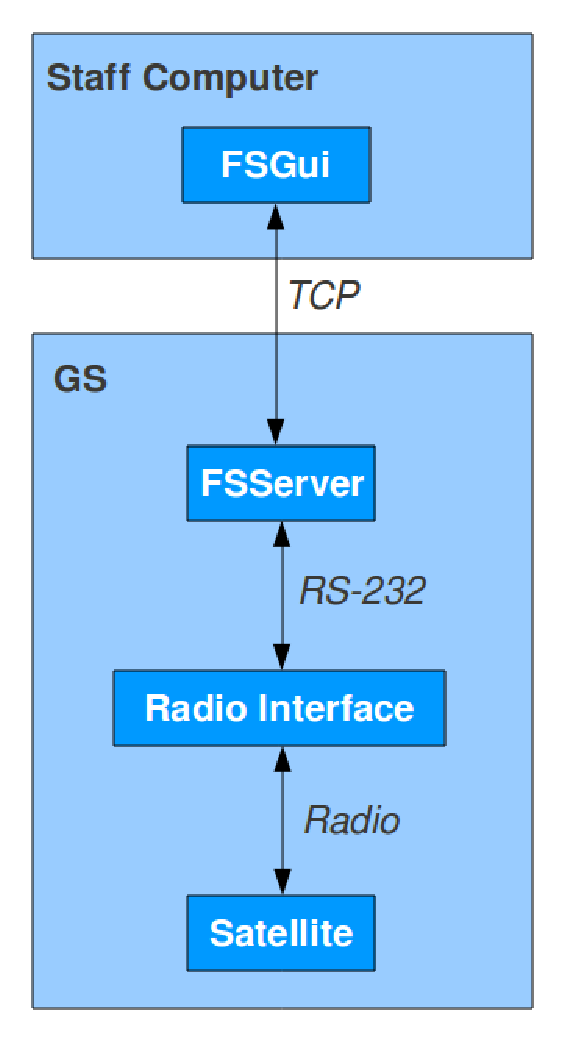
\includegraphics[scale=0.5]{img/tcp_interface_to_the_radio}
  \caption{TCP Interface to the radio}
\end{figure}

\subsection{Command Combinations}
The failsafe software has a set of basic commands which by themselves are of limited use but becomes powerful when combined. As we cannot know which failures might occur in the future, it is critical that there is a flexible way of combining these commands in conditionals and loops.

One solution is to combine the commands in the GUI. Then we would need to construct individual GUI elements for concepts like a command, a command sequence, an if statement and its branches, a loop statement and its body and so forth. This solution is hard to extend with a switch-statement in two years time when someone needs it - and impossible to do without the source code.

The use of script languages to combine commands
Alternatively there is a far more flexible solution to this challenge when it is recognized that conditionals and loops already have been implemented numerous times in script languages such as Ruby, Python or TCL and that they can be used to achieve the required flexibility.

Send failsafe commands from a script using UNIX
It is necessary that the scripts can communicate with the Ground Station. To solve this each script could implement a TCP client, but that would mean two things. One, a TCP client for each specific language would be needed before they could be used to write failsafe scripts. This is inflexible. Two, there would exist several implementation of the TCP client which is error-prone.

Is there anything all scripting languages have in common? Well, if we assume that the scripts are being run on a UNIX system, they will have exactly that in common. All languages have built-in libraries for running a UNIX console command and manipulating the output. So, we could use fsclient to pass failsafe commands through. Fsclient will just handle the TCP connection to the Ground Station and forward the commands.

FSServer must be aware of multiple TCP clients and ensure that commands from various TCP clients are not executed at the same time. This challenge is covered the chapter \ref{chap:fsserver}.

\begin{figure}[h!] \centering
	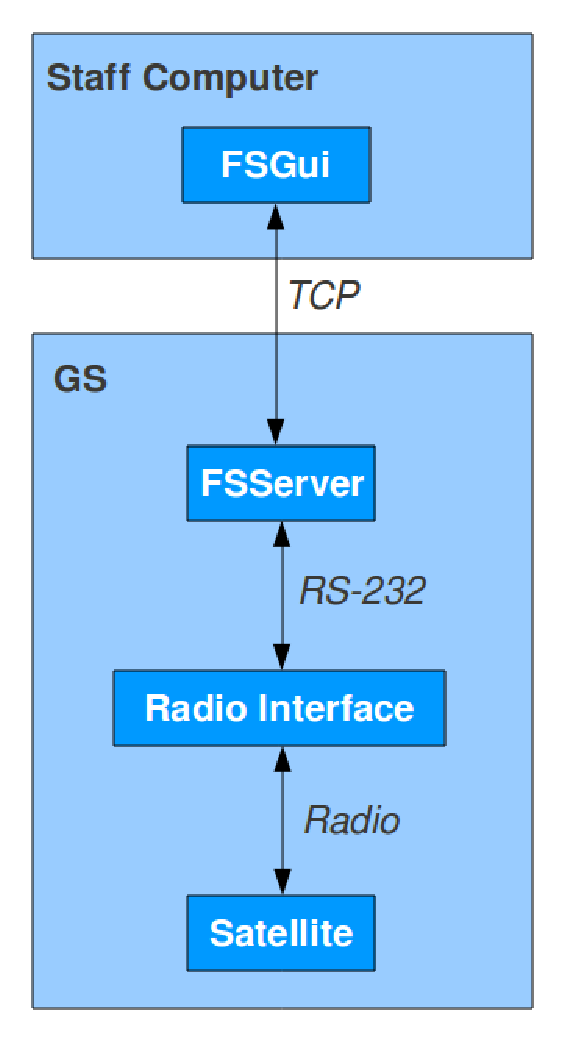
\includegraphics[scale=0.5]{img/tcp_interface_to_the_radio}
  \caption{FSClient and executing scripts}
\end{figure}

\subsection{Graphical representation of the health status}
The failsafe software has a command called HEALTH\_STATUS which will return a set of numbers representing the state of the subsystems. These numbers will be interpreted as temperature, current and voltage values in the GUI. The GUI must provide a graphical representation of the subsystems and their health status.

\section{Chosen design}
Here is a wrap up of the final design that consists of four key elements:

\textbf{FSServer}
\begin{itemize}
	\item Installed on GS
	\item A TCP server
	\item Send failsafe commands via the datalink
	\item Send failsafe response back to TCP clients
	\item Ensure atomicity of failsafe commands
\end{itemize}

\textbf{FSClient}
\begin{itemize}
	\item Installed on the staff's desktop computers
	\item Unix program
	\item A TCP client to FSServer
	\item Forward failsafe commands from other unix programs to the server
	\item Interactive mode
\end{itemize}

\textbf{FSGui}
\begin{itemize}
	\item Installed on the staff's desktop computers
	\item Runs on unix and windows systems
	\item A TCP client to FSServer
	\item No installation required, just download and double-clik
	\item Create, save, load, export command sequences
	\item Execute failsafe scritps
	\item View graphical representation of the health status
\end{itemize}

\textbf{Scripts}
\begin{itemize}
	\item Any script or programming language that can execute unix commands
	\item Combine failsafe commands in conditionals and loops
\end{itemize}

\begin{figure}[h!] \centering
	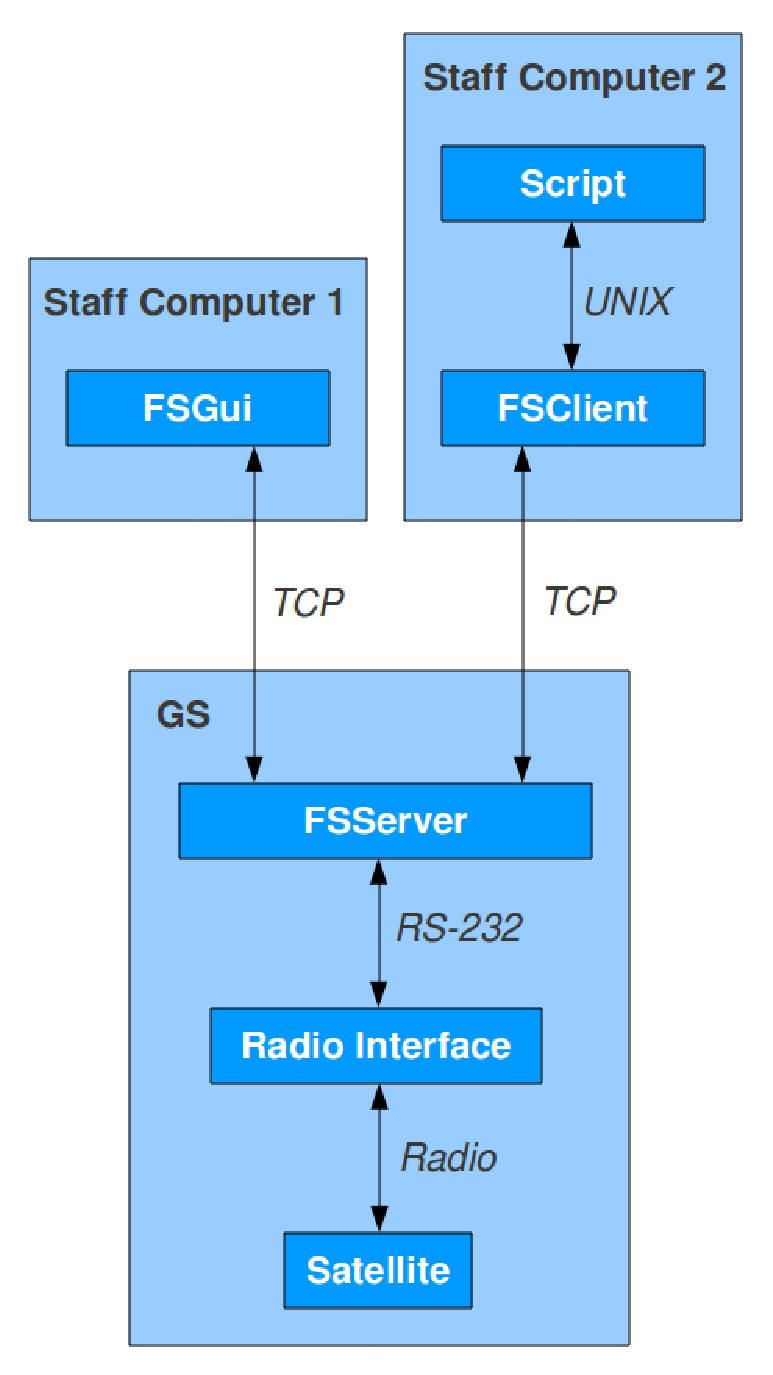
\includegraphics[scale=0.5]{img/chosen_design}
  \caption{The chosen design}
\end{figure}

Now that there is an overall design, lets proceed with an analysis, design and implementation part of the individual parts.
